\chapter{Regiões Densas Interessantes (IDRs)}
\label{chap:idrs}

Neste capítulo explana-se mais profundamente o conceito de Regiões Densas Interessantes e qual a sua utilidade em uma análise de dados espaciais. Também será detalhado o passo a passo para a criação de uma Região desse tipo, qual a função do feedback do usuário nessa construção, qual o algoritmo usado para esse processo, qual sua utilização no GeoGuide e quais as vantagens que podemos obter quando utilizamos Regiões Densas Interessantes para fazer análise de dados espaciais com uma abordagem de orientação do usuário através da ferramenta.

\section{Feedback do usuário}

Para poder explicar melhor o conceito de IDR, precisamos começar falando sobre o \textit{feedback} do usuário, como funciona e como isso pode ser utilizado na criação das Regiões. Durante a utilização de um sistema, o usuário vai interagindo com suas funcionalidades e o sistema vai respondendo aos seus comandos e ações, isso faz com que um sistema seja interativo e dinâmico, podendo ser atualizado conforme o usuário e as características de cada um. Em sistemas de análise de dados espaciais, é muito comum que seja utilizado um mapa, um gráfico ou qualquer recuso visual que facilite a interpretação do usuário e dê uma noção sobre o que se trata o dataset em si.

A partir disso, o usuário pode ir ``caminhando'' pelo mapa (ou figura) para ir conhecendo mais afundo os dados e as particularidades de cada ponto. Esse ``caminhar'' pode se tornar interessante para o sistema de forma que isso ajude a conhecer os interesses do usuário. Essa resposta que o usuário concede ao sistema enquanto o estar utlizando, é o que caracteriza o \textit{feedback} e isso pode trazer muitas utilizações para diversos tipos de sistemas.

O feedback pode ser dividido em duas categorias sobre a abordagem utilizada para sua coleta: o \textit{explícito} e o \textit{implícito}. O primeiro se refere a quando o usuário define como interessante de forma consciente utilizando meios que o próprio sistema indica como funciona e para que serve. Por exemplo: quando o usuário indica se gostou de determinada indicação, quando ele vota de 0 a 5 estrelas num filme de sua preferência, quando ele indica algum restaurante para alguém utilizando o sistema, quando ele clica num ponto no mapa para obter mais informações e de várias outras formas pode se obter um feedback explícito.

Já no caso da segunda categoria de feedback, o usuário não precisa dizer diretamente qual o seu interesse no sistema, do contrário, o sistema vai detectando progressivamente o que o usuário vai fazendo na plataforma e vai registrando isso para, a partir de uma determinada quantidade de informação, conseguir caracterizar algo como interessante para o usuário. Por exemplo, o sistema pode rastrear o movimento do mouse ou dos olhos para conseguir definir onde o usuário mais foca no sistema durante sua utilização, para isso ele precisa registrar os pontos rastreados do usuário e ir salvando isso. Então, com uma grande coleção de pontos, o sistema pode utilizar algoritmos de clusterização para encontrar as áreas mais marcantes desse conjunto e classificar elas como de interesse do usuário.

Esse tipo de feedback implícito é utilizado no GeoGuide para a captura de interesse do usuário através do rastreamento do mouse e utilizando algoritmos de clusterização para construir essas áreas que consideramos de interesse do usuário durante sua exploração pelo mapa da plataforma. Tudo isso de forma que o usuário não saiba e não precisa gastar nenhum esforço para indicar o que lhe é interessante, somente usando a plataforma já podemos detectar essa informação.

\section{Regiões no GeoGuide}

Como dito anteriormente, o feedback que o usuário entrega ao sistema é de extremo valor para o aprimoramento da ferramenta e das análises que ela performar. Isso faz com que a ferramenta tenha a característica de se adequar a cada usuário e trazer o melhor resultado para cada um em específico. Também foi abordado que no GeoGuide utilizamos o feedback implícito do rastreamento do mouse para detectar as áreas de interesse do usuário.

Entretanto, adicionamos o conceito de IDR para ir mais além nessa detecção e aprimorar a análise do usuário reforçando alguns aspectos que somente com áreas isoladas não iríamos conseguir. Esse conceito de Regiões Densas Interessantes é baseado na detecção de áreas de interesse do usuário construídas a partir do rastreamento do seu mouse.

No GeoGuide, registramos o movimento do mouse do analista durante um determinado intervalo de tempo e os separamos em diferentes conjuntos (na Figura \ref{fig:idrs-geoguide}.A podemos ver o registro de 3 momentos diferentes do movimento do mouse). Para cada conjunto, nós realizamos a clusterização desses pontos para a formação das áreas de interesse. Cada área é representada por um conjunto de pontos agrupados por sua proximidade em relação de um aos outros.

A partir desse conjunto, construímos um polígono convexo utilizando os pontos mais distantes do centro (podemos ver um exemplo disso na Figura \ref{fig:idrs-geoguide}.B). Cada polígono é a representação da área de interesse do usuário. Isto posto, para a formação de uma IDR, nós dividimos uma quantidade de momentos de formação dos polígonos (as Figuras \ref{fig:idrs-geoguide}.B, \ref{fig:idrs-geoguide} C e \ref{fig:idrs-geoguide}.D representam as formações de áreas de interesse em 3 momentos diferentes consecutivos) e definimos como IDR a interseção desses polígonos entre si (podemos ver um exemplo na Figura \ref{fig:idrs-geoguide}.E marcado pela área de fundo preto quadriculado). Ou seja, na nossa ferramenta, decidimos que a cada 20 segundos de rastreamento do mouse, o sistema vai construir uma pequena série de polígonos formados a partir do cluster desses pontos de rastreio e registrar para o próximo passo. Após 3 momentos de construção de clusters, nós selecionamos todos os polígonos resultantes e calculamos novos polígonos formados pela interseção das áreas de cada momento (na Figura \ref{fig:idrs-geoguide}.F podemos ver a formação de 4 IDRs a partir das interseções das áreas da Figura \ref{fig:idrs-geoguide}.E). Este processo se repete enquanto o analista estiver utilizando a ferramenta.

\begin{figure*}[t]
	\centering
	\includegraphics[width=\textwidth]{images/idrs}
	\caption{Figura do processo de construção de IDRs}
	\label{fig:idrs-geoguide}
	\vspace{-10pt}
\end{figure*}

O resultado dessas interseções são o que chamamos de Regiões Densas Interessantes, e isso torna a formação da área de interesse do usuário mais reforçada e precisa, pois cada IDR vai demonstrar uma região que o usuário focou em mais de um momento em tempos diferentes.

\begin{figure*}[t]
	\centering
	\includegraphics[width=\textwidth]{images/idrs-matching.pdf}
	\caption{Figura das sugestões do GeoGuide relacionadas com as IDRs do analista}
	\label{fig:idrs}
	\vspace{-10pt}
\end{figure*}

Por exemplo, um analista está explorando o dataset do Airbnb e deseja encontrar novas sugestões de residências. Durante sua exploração foram geradas 4 IDRs e então ele requisitou ao GeoGuide o \textit{highlight} de novos pontos e para o resultado foi levado em consideração as IDRs resultantes de sua exploração. Como podemos ver na Figura \ref{fig:idrs}, os pontos sugeridos pelo GeoGuide estavam em 3 das 4 regiões do analista e isso reforça o interesse dele naquelas regiões.

Com isso, cada IDR pode ser utilizada tanto para um foco mais preciso na região,caso queira restringir mais o escopo da análise, quanto para diminuir as sugestões nessa região e assim abrir mais o leque de opções do analista e expandir sua área de pesquisa, incrementando novas possibilidades para sua análise.

\section{Algoritmo}

Nós consideramos duas camadas diferentes no mapa geográfico: a ``camada espacial'' e a ``camada de interação''. A camada espacial contém os pontos espaciais $\mathcal{P}$ do dataset em análise. A camada de interação  contém os pontos $\mathcal{M}$ referente aos pontos de movimento do mouse. Nossa abordagem proposta foca um conjunto dos pontos $\mathcal{M}$ na camada de interação para descobrir uma ou mais IDRs, na qual a maioria das interações do analista ocorre. Então alinhamos os pontos espaciais $\mathcal{P}$ com as IDRs visando encontrar os pontos que estão dentro de cada região. 

\begin{algorithm}[!h]
        \DontPrintSemicolon
        \KwIn{Tempo atual $t_c$, pontos dos movimentos do mouse $\mathcal{M}$}
        \KwOut{IDRs encontradas $\mathcal{S}$}
        $\mathcal{S} \gets \emptyset$\;
        $g \gets ${\em número de intervalos}\;
        \For{$i \in [0,g]$}
        {
               $\mathcal{M}_i \gets \{m = \langle x,y,t \rangle | (\frac{t_c}{g} \times i) \leq t \leq (\frac{t_c}{g} \times (i+1))\}$\;
               $\mathcal{C}_i \gets \mathit{minerar\_clusters}(\mathcal{M}_i)$\label{ln:mine}\;
               $\mathcal{O}_i \gets \mathit{encontrar\_poligonos}(\mathcal{C}_i)$\label{ln:poly}\;
        }
        \lFor{$\mathcal{O}_i, \mathcal{O}_j$ onde $i,j \in [0,g]$ e $i \neq j$}
        {
            $\mathcal{S}.\mathit{append}(\mathit{intersect}(\mathcal{O}_i, \mathcal{O}_j))$
        }
        \Return{$\mathcal{S}$}\;  
        \caption{Algoritmo para criação de IDRs}
        \label{algo:dense}
\end{algorithm}

O algoritmo \ref{algo:dense} resume nossa abordagem para encontrar as IDRs. Nós adicionamos pontos para o conjunto $\mathcal{M}$ somente a cada $200ms$ para evitar a adição de pontos repetidos. Seguindo a ideia de que o analista tem mais interesse naquela região se ele movimentar o mouse nela mais vezes e afim de minerar o comportamento recorrente do analista, o algoritmo começa pelo particionamento do conjunto $\mathcal{M}$ em $g$ segmentos consecutivos de tamanho fixo do $\mathcal{M}_0$ até o $\mathcal{M}_g$. O primeiro segmento inicia no tempo zero (quando o usuário abre o mapa) e o último segmento termina em $t_c$, ou seja, o momento atual. Baseado na ideia de que o analista pode percorrer o mapa completamente, mas isso não indicará seu real interesse por todo o mapa, nós buscamos encontrar os clusters mais densos de cada segmento do conjunto $\mathcal{M}$ utilizando um algoritmo variante do DBSCAN \cite{Ester:1996:DAD:3001460.3001507}. Por fim, nós retornamos as interseções entre esses clusters como os IDRs.

Para clusterizar os pontos em cada segmento de tempo (linha \ref{ln:mine} do Algoritmo \ref{algo:dense}), nós usamos o ST-DBSCAN, um variante do DBSCAN para clusterizar pontos baseado na sua densidade \cite{Birant:2007}. Para cada subconjunto dos pontos do movimento do mouse $\mathcal{M}_i$, $i \in [0,g]$, o ST-DBSCAN inicia com um ponto aleatório $m_0 \in \mathcal{M}_i$ e coleciona todos os pontos ``densamente alcansáveis'' de $m_0$ usando uma métrica de distância. Como os pontos do movimento do mouse estão numa tela de 2 dimensões (isto é, o monitor), nós escolhemos a distância euclidiana como nossa métrica. Se $m_0$ for considerado um ponto central,  um cluster será gerado. Do contrário, se o $m_0$ for um ``ponto de borda'', nenhum ponto é alcançado por ele e o algoritmo escolherá outro ponto aleatório em $\mathcal{M}_i$. O processo é repetido até que todos os pontos tenham sido processados e categorizados.

Uma vez que encontramos os clusters de todos os subconjuntos de $\mathcal{M}$, nós encontramos suas interseções para encontrar regiões recorrentes (linha \ref{ln:poly}). Para obter as interseções, nós precisamos definir claramente os limites espaciais de cada cluster. Por isso, para cada cluster nós definimos um polígono correspondente que cubra todos os pontos dentro. Para conseguir isso, nós utilizamos o algoritmo Quickhull \cite{Barber:1996}, um método parecido com o \textit{quicksort} que calcula um polígono convexo para um determinado conjunto de pontos num plano 2D.

Já existem diversas formas de inferir uma região espacial para um determinado conjunto de pontos \cite{Bevis1989,DUCKHAM2008,FADILI2004,ARAMPATZIS2006,Galton2006}. A abordagem comum é agrupar os pontos em forma de polígonos concavos e convexos. Nos casos em que um polígono côncavo é construído, os ``dentes'' desse polígono podem vincular pontos que não necessariamente estariam em $\mathcal{M}$. No algoritmo de IDR, entretanto, nós adaptamos o Quickhull devido a sua simplicidade, eficiência e implementação padrão para polígonos convexos.

\section{Sequência de Processamento de IDRs e Outliers no GeoGuide}

Nesta seção iremos mostrar como utilizar os conceitos de IDRs e a abordagem de detecção de outliers no GeoGuide. Será mostrado o passo a passo de como utilizar a plataforma do GeoGuide, desde o passo da autenticação, passando pelo processo \textit{upload} de um dataset no formato \textit{csv}, apresentando como o GeoGuide trata esse conjunto de dados e então exemplificando a criação de IDRs na plataforma e a abordagem de detecção de outliers nesse conjunto.

\subsection{Carregando um dataset}

O primeiro passo para começar a utilizar o GeoGuide é realizar um cadastro básico do usuário (informando os campos \textit{e-mail}, \textit{senha} e \textit{confirmação de senha}) que está acessando a plataforma (ver Figura \ref{fig:geoguide-register}). Caso o usuário já possua conta na plataforma, então ele só precisará informar seu email e senha que usou durante o cadastro para poder ter acesso ao GeoGuide (ver Figura \ref{fig:geoguide-login}).

\begin{figure*}[h]
	\centering
	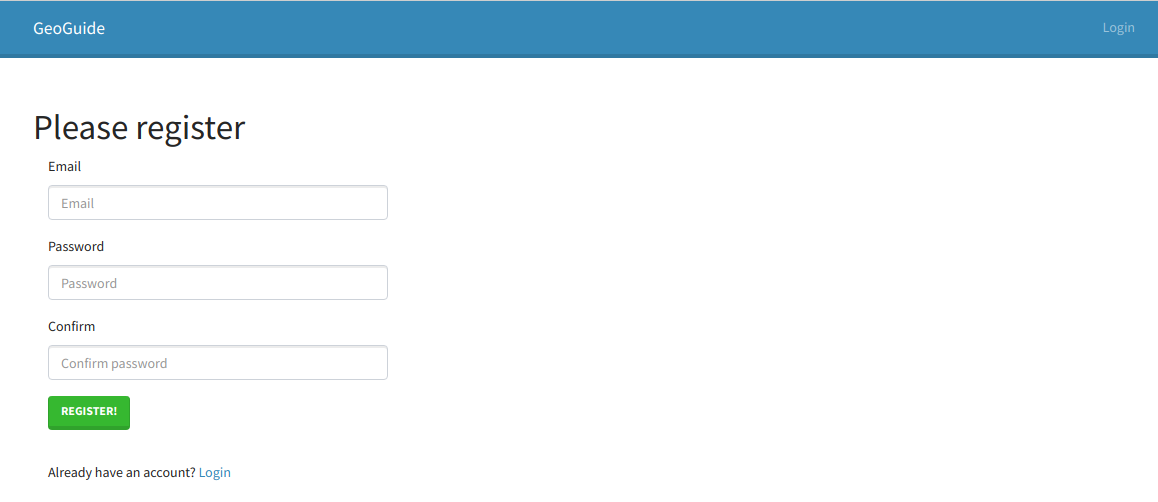
\includegraphics[width=\textwidth]{images/geoguide-register.png}
	\caption{Tela de registro de usuário do GeoGuide}
	\label{fig:geoguide-register}
	\vspace{-10pt}
\end{figure*}

Esse cadastro é importante para que o usuário possa registrar os datasets carregados e não precisar ficar fazendo o mesmo carregamento desses dados várias vezes, pois todas as suas configurações vão ficar registradas na plataforma e ligadas diretamente à sua conta de usuário.

\begin{figure*}[h]
	\centering
	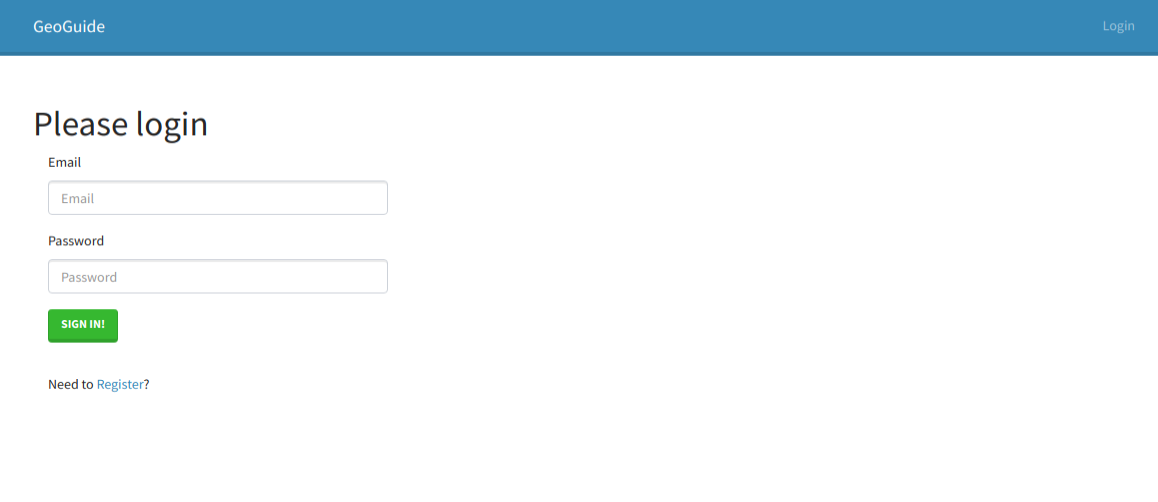
\includegraphics[width=\textwidth]{images/geoguide-login.png}
	\caption{Tela de login do usuário do GeoGuide}
	\label{fig:geoguide-login}
	\vspace{-10pt}
\end{figure*}

Após escolher qual conjunto de dados ele vai querer trabalhar, é preciso que ele realize o processo de carregamento de um arquivo .csv e então informar alguns dados básicos sobre aquele conjunto que vai estar registrando na sua conta, como por exemplo: qual o nome que ele vai atribuir àquele conjunto, quantas linhas do .csv vai levar em consideração no carregamento (isso é importante para caso o usuário deseje analisar somente uma parte do dataset), quais os campos que ele quer levar em consideração para o cálculo das métricas de \textit{similaridade} \textit{diversidade} e entre outras informações.

\begin{figure*}[h]
	\centering
	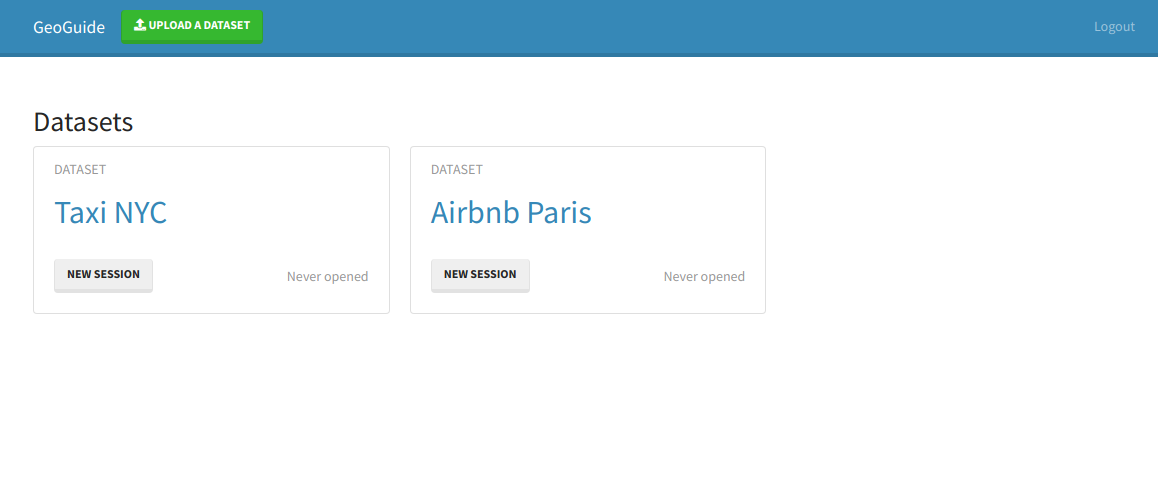
\includegraphics[width=\textwidth]{images/geoguide-datasets.png}
	\caption{Tela de datasets do usuário no GeoGuide}
	\label{fig:geoguide-datasets}
	\vspace{-10pt}
\end{figure*}

Quando finalizar o preenchimento do formulário referente ao dataset, então o analista poderá visualizar quais os datasets que já estão registrados na sua conta e selecionar qual ele irá querer trabalhar no momento. Após isso, o GeoGuide passará para o próximo passo que é a visualização desses dados espaciais num mapa global centralizado na localização do dataset, de forma que o usuário já possa interagir com os pontos no mapa, podendo realizar algumas filtragens e também clicando em cada ponto específico para mostrar seus atributos referentes ao seu domínio específico.

\subsection{Pré-processamento do GeoGuide}

Logo após o primeiro instante de plotagem do mapa global na tela do usuário, o servidor da plataforma do GeoGuide inicia, em paralelo e sem a intervenção do usuário, um processo para o cálculo das métricas de similaridade e diversidade de todos os pares de pontos possíveis no dataset.

Primeiro a ferramenta seleciona um ponto $a$ do dataset espacial e o compara com um ponto $b$ sendo seu sucessor no conjunto. A comparação leva em consideração os atributos ``não espaciais'' dos pontos e tem como resultado a métrica de \textit{similaridade} entre esses dois pontos. Então, é realizado uma segunda comparação para gerar a métrica de \textit{diversidade} entre os pontos. Para essa métrica, é levado em consideração os atributos geográficos desses pontos (\textit{latitude} e \textit{longitude}), de forma que, quanto mais distante um ponto $a$ é do ponto $b$, mais diverso eles serão.  

\begin{figure*}[h]
	\centering
	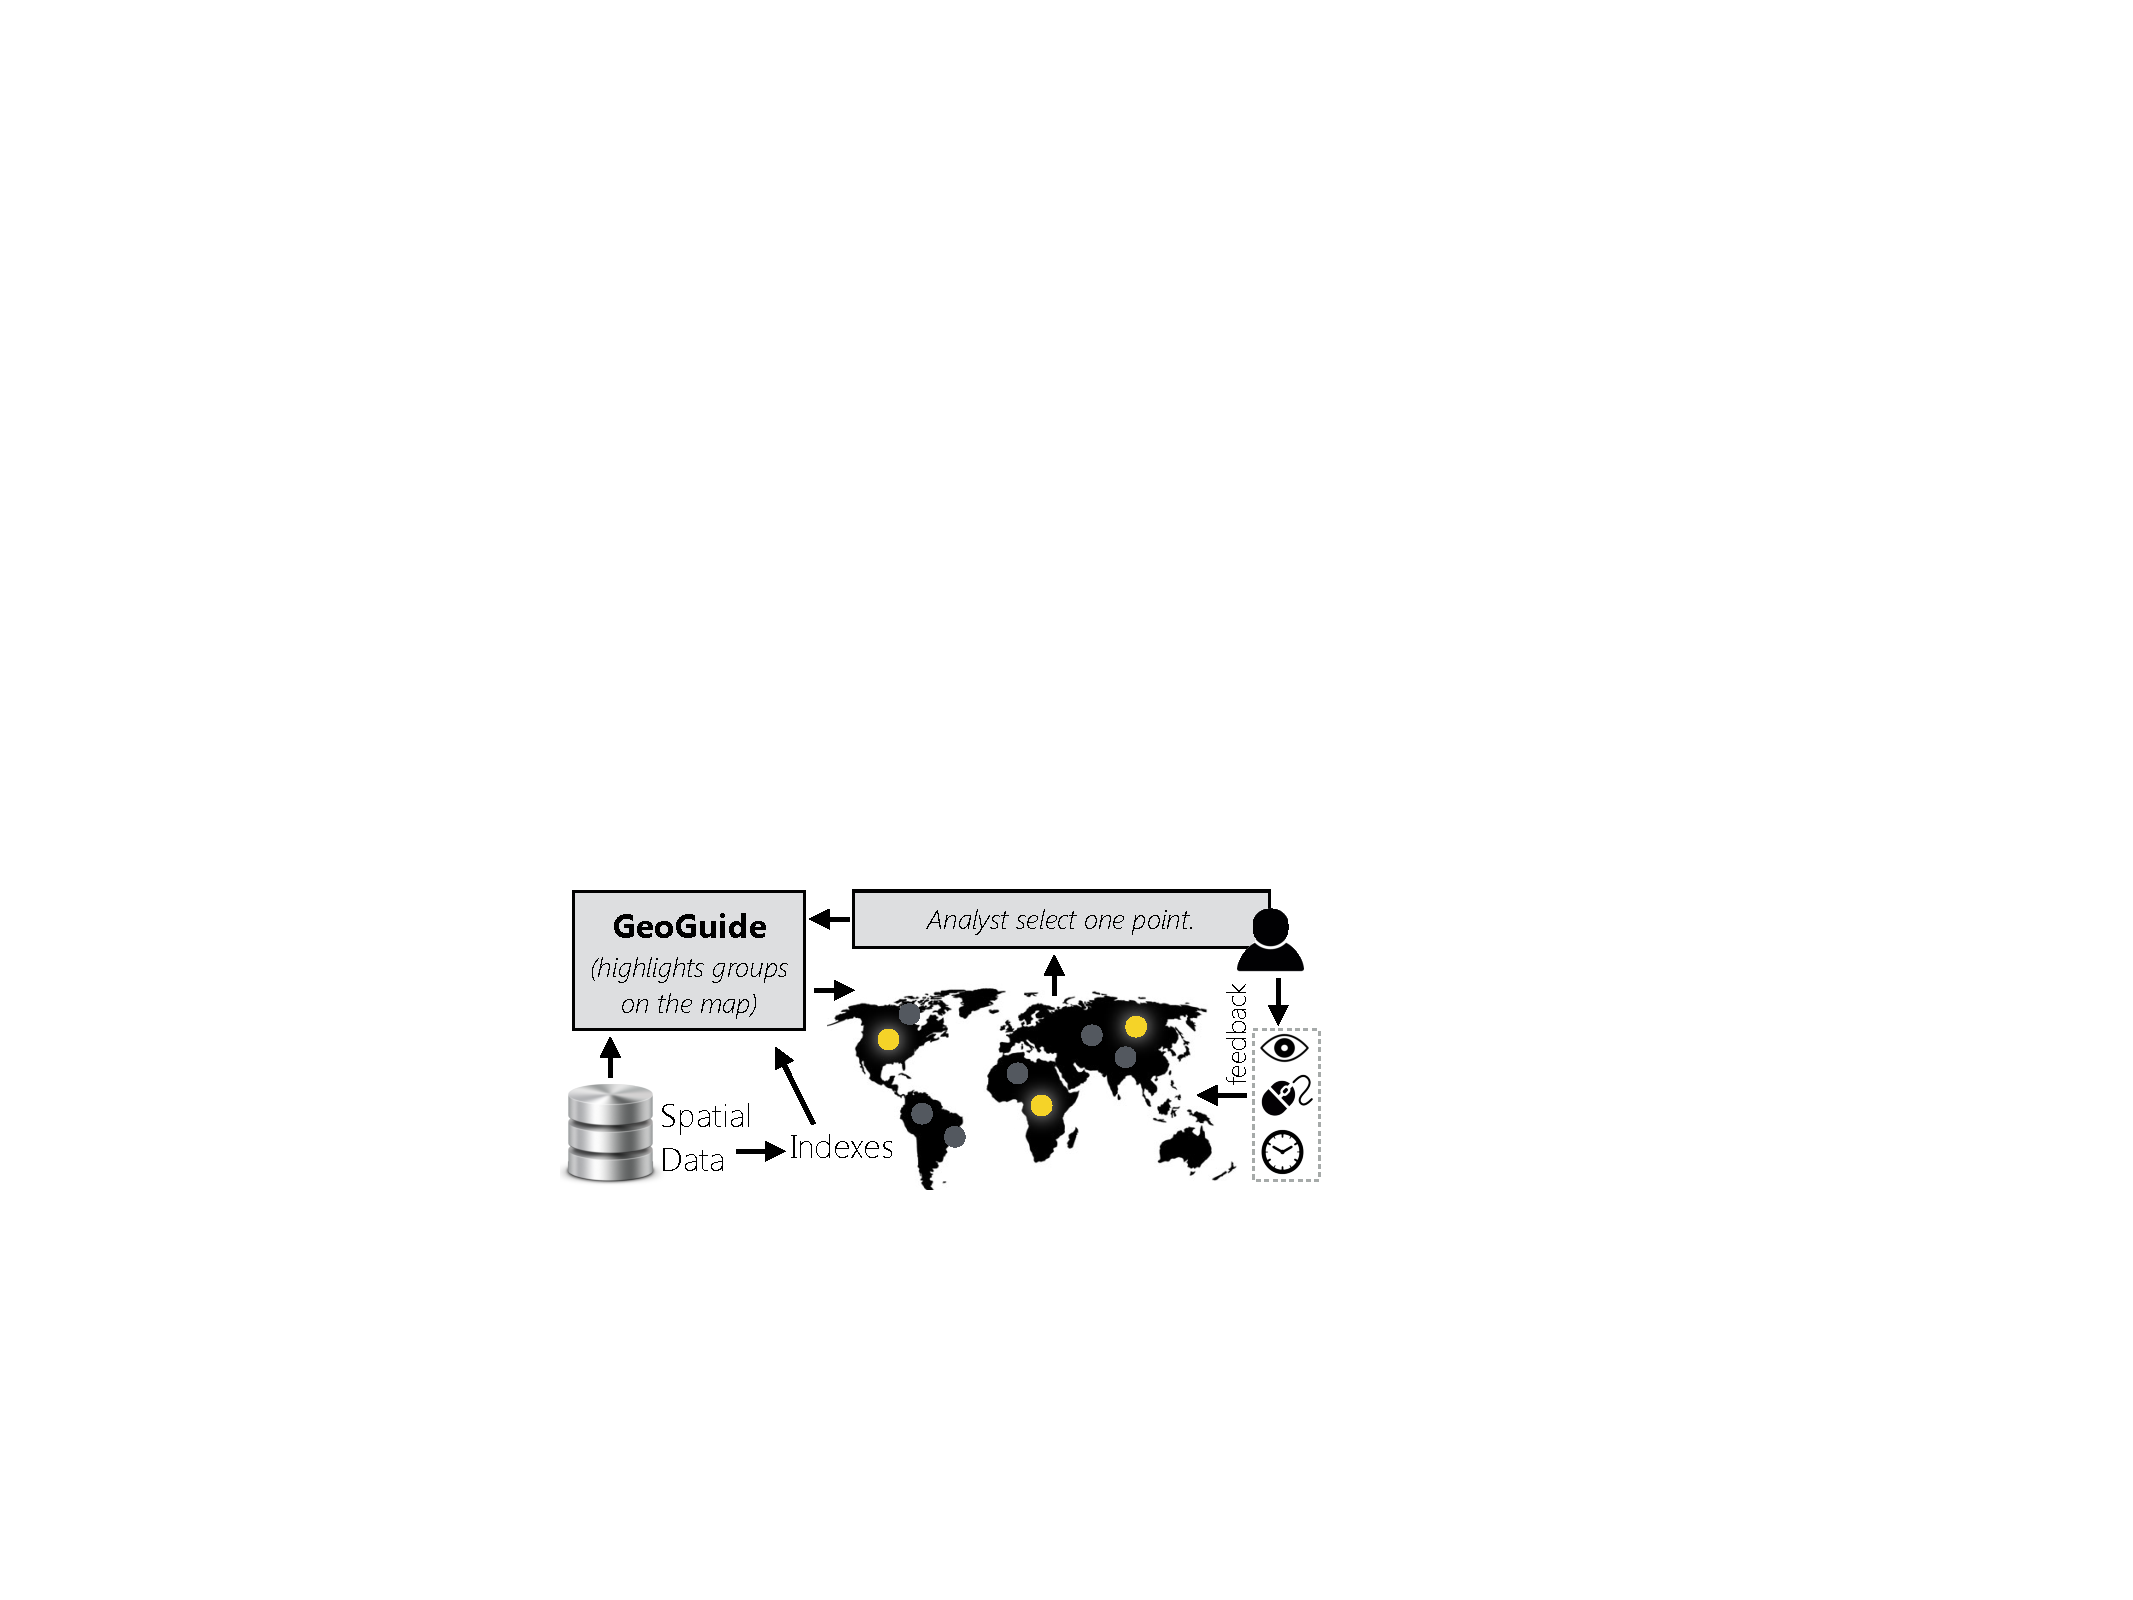
\includegraphics[width=\textwidth]{images/geoguide-pre-processamento.pdf}
	\caption{Visão geral do funcionamento do GeoGuide}
	\label{fig:geoguide-pre-processamento}
	\vspace{-10pt}
\end{figure*}

Após o processamento dessas métricas, o framework vai normalizar esses valores num intervalo de $0,0$ a $1,0$ e orderná-los em sentido decrescente. Esses valores normalizados são os indíces (ver Figura \ref{fig:geoguide-pre-processamento}) que o GeoGuide utilizará nas sugestões de novos pontos para o analista.

Esse processo é demorado, pois tem a complexidade de $\mathcal{O}(n^{2})$ e isso vira um problema com o aumento do volume desses datasets. Então durante esse cálculo o usuário pode ir navegando pelo seu conjunto de dados e ir conhecendo mais sobre os pontos daquele grupo (gerando \textit{feedback} para a ferramenta, como podemos ver na Figura \ref{fig:geoguide-pre-processamento}). Quando for de seu interesse, o analista pode selecionar um ponto e pedir novas sugestões relacionadas com sua escolha, logo, o GeoGuide irá consultar os indíces resultantes do seu processamento inicial e retornará os pontos mais relevantes com a escolha do usuário. Esse processo pode ser realizado diversas vezes para que o analista sempre possa descobrir o que explorar em seguida.

\subsection{Criação de IDRs}

No mesmo momento que o servidor da plataforma é disparado para realizar o pré-processamento do dataset para gerar os indíces normalizados das métricas principais do GeoGuide, a aplicação do usuário, quando concluir a plotagem do mapa, começará o processo de rastreamento do movimento do mouse.

Como dito anteriormente, essa coleta dos pontos do mouse usuário navegando a plataforma é importante para a criação dos IDRs e sua utilização nas orientações que o GeoGuide vai propor baseado num ponto escolhido pelo usuário. Essa criação de IDRs obedece os intervalos de $20$ segundos para o processo de clusterização dos pontos, utilizando o algoritmo \textit{k-means} para a criação desses clusters, e também o intervalo definido previamente de que, após $3$ momentos de clusterização, serão selecionados os polígonos resultantes da interseção dos clusters de cada momento e isso resultará nas áreas definidas como IDRs.

Esse processo de construção das IDRs acontece todo o tempo em que o usuário esteja utilizando a plataforma e, a cada geração de IDR, essas regiões serão enviadas para o servidor registrando de qual usuário é essa IDR e qual a seção dele no momento de construção. Com essas informações é então possível ter um histórico das regiões de interesse do usuário e usar esses dados para um outro tipo de análise de preferência do usuário levando em consideração outros fatores.

Todo essa operação mostra a importância das criações das IDRs e também demonstra que as aplicações desses dados podem se expandir, dependendo somente de qual a necessidade que se quer suprir com essas informações.

\subsection{Detectando Outliers}

Com a construção das IDRs acontecendo durante a utilização do GeoGuide pelo usuário, um outro processo também é executado após cada momento de criação dessas regiões. Com cada região encontrada, nós selecionamos os pontos que estão inseridos em cada região e para cada grupo desse efetuamos uma detecção de outliers nessa região levando em consideração os atributos definidos pelo usuário durante o carregamento desse dataset.

Dessa forma, além de registrar a cada minuto quais são as áreas que o usuário tem mais interesse baseado no seu movimento de mouse, nós também gravamos quais são os pontos considerados discrepantes de cada região dessa e, com isso, temos os dados suficientes para o processo final das orientações que o GeoGuide performará quando requerido pelo usuário.

\subsection{Processamento final}

Desde o momento que o usuário é imerso no mapa global com os pontos de seus datasets plotados, as ações que acontecem são desconhecidas pelo usuário e acontecem sem sua menor interferência ou sem ele conseguir notar seu processamento.

Porém, o momento mais importante para o usuário e que é finalidade de todo esse processo executado em \textit{background}, é quando ele seleciona um ponto de seu interesse e então pede $k$ novos pontos como sugestões do GeoGuide baseado nos atributos do ponto escolhido pelo usuário. Nesse momento é que será levado em consideração as IDRs registradas na sua seção e os outliers detectados em cada região.

Agora, nessa nova proposta do GeoGuide, os pontos que se encontrarem dentro das regiões definidas como IDRs pelo usuário serão priorizados para serem sugeridos, pois assim o usuário conseguirá obter mais informações dentro de uma região que já é previamente definida como interessante para ele e não irá perder seu foco em outras possíveis regiões.

E também, no momento em que o GeoGuide propõe novos pontos para serem analisados, os pontos registrados como outliers dentro das IDRs também serão privilegiados nessa proposta do GeoGuide, pois, como visto em outra pesquisa \cite{DBLP:journals/debu/FreireCVZ16}, esses pontos ``aberrantes'' podem indicar novas características desse dataset e um começo de por onde procurar particularidades desse dataset escolhido pelo usuário.
